\chapter{Theory}\label{chapter:theory}
\section{The Standard Model}\label{sec:sm}
The Standard Model (SM) of particle physics is a Quantum Field Theory (QFT) which describes all the known elementary matter particles and their interactions with the weak, strong, and electromagnetic forces.
As a QFT, particles are described as excitations of quantum fields whose dynamics are typically described using the Lagrangian formalism~\cite{LagrangiansSM}.

This chapter introduces and briefly describes the theoretical framework of the SM, the physics of top quark and the shortcomings of the SM.
The second section of the chapter discusses the motivations and context of the search for a single top quark produced in association with a Z boson presented in this thesis.

Throughout this thesis \emph{natural units} where the fundamental constants $c$, $\hbar$ and $k_{B}$ are equal to unity, and Einstein's summation convention are used.

\subsection{Fundamental Particles}\label{subsec:particles}
The SM describes all matter as spin-$\frac{1}{2}$ particles known as fermions which interact through the fundamental forces which are mediated by spin-$1$ gauge bosons.
The spin-$0$ Higgs boson arises as a consequence of the electroweak symmetry breaking as a means to imbue the fermions and weak force gauge bosons with mass.

Matter consists of six quarks, particles which interact through the strong, electromagnetic and weak forces, and six leptons, particles which experience the electromagnetic and weak forces~\cite{LagrangiansSM}.
Each fermion has an associated anti-matter equivalent which has an identical mass but opposite charge.
Both types of fermion are subdivided into three ``generations'' of particles where each subsequent generation of particles is identical, except for their quantum number and mass~\cite{ElectroweakStrong}.
Table~\ref{tab:fermions} lists the charges, weak isospins and masses of the quarks and leptons for each of the three generations.

The ``up-type'' and ``down-type'' quarks of each generation have both an electrical charge of $\frac{+2}{3}$ and $\frac{-1}{3}$  respectively and a \emph{colour charge} (or anti-colour charge) of red, blue or green.
As the phenomena of \emph{colour confinement} (as described below in Section~\ref{subsec:QCD}) only allows for colourless states, quarks form composite particles called hadrons.
Typically hadrons are composed of a quark anti-quark pair, collectively termed mesons, or of three quarks, referred to as baryons.
Exotic hadrons formed of larger groupings of quarks can be also formed, with both tetraquark and pentaquark states being observed and discovered, respectively, by the LHCb detector~\cite{Aaij:2014jqa,Aaij:2015tga}.

Each generation of leptons consist of a charged lepton which interacts through the electromagnetic and weak forces, and a corresponding neutral near massless lepton, known as a neutrino, which interacts solely through the weak force.
As with the quarks, the charged lepton of each subsequent generation is more massive than the last.
Initially the SM assumed that neutrinos were massless, but the discovery of neutrino flavour oscillation implies that they have a non-zero mass. 
It is currently unknown whether the hierarchy of the neutrino mass eigenstates is analogous to that of the charged lepton or otherwise~\cite{Nath:2018rqn}.

\begin{table}[htbp]
\topcaption {
The Standard Model fermions and their properties.
}
\label{tab:fermions}
  \centering
  \resizebox{\textwidth}{!}{
% This right-aligns numbers in column, but centers them under column title.
 \begin{tabular}{llcllccc}
   \hline
   & \textbf{Generation} & \textbf{Particle} & & \textbf{Mass \MeV} & \textbf{Electric Charge} & \textbf{Colour Charge} & \textbf{Weak Isospin}\\
   \hline
   \multirow{3}{*}{Quarks}  & \multirow{2}{*}{I} & up \textit{$u$}  & 2.3 & $+ \frac{2}{3}$ & 0 & $+ \frac{1}{2}$ \\
   & & down & \textit{$d$} & $4.8$ & $- \frac{1}{3}$ & $0$ & $- \frac{1}{2}$ \\
   & \multirow{2}{*}{II} & charm & \textit{$c$}  & $2.3$ & $+ \frac{2}{3}$ & 0 & $+ \frac{1}{2}$ \\
   & & strange & \textit{$s$}  & $4.8$ & $- \frac{1}{3}$ & $0$ & $- \frac{1}{2}$ \\
   & \multirow{2}{*}{II} & top & \textit{$t$}  & $2.3$ & $+ \frac{2}{3}$ & $0$ & $+ \frac{1}{2}$ \\
   & & bottom &\textit{$b$}  & $4.8$ & $- \frac{1}{3}$ & $0$ & $- \frac{1}{2}$ \\
   \hline
   \multirow{3}{*}{Leptons}  & \multirow{2}{*}{I} & electron \textit{$e$}  & $0.511$ & $-1$ & $0$ & $- \frac{1}{2}$ \\
   & & electron neutrino & \textit{$\nu_{e}$}  & $< 2 \times 10^{-6}$ & $0$ & $0$ & $+ \frac{1}{2}$ \\
   & \multirow{2}{*}{II} & muon & \textit{$\mu$}  & $106$ & $-1$ & $0$ & $-\frac{1}{2}$ \\
   & & muon neutrino & \textit{$\nu_{\mu}$}  & $< 0.19$ & $0$ & $0$ & $+ \frac{1}{2}$ \\
   & \multirow{2}{*}{II} & tau & \textit{$\tau$}  & $1777$ & $0$ & $0$ & $- \frac{1}{2}$ \\
   & & tau neutrino & \textit{$\nu_{\tau}$}  & $<18.2$ & $0$ & $0$ & $+ \frac{1}{2}$ \\   
   \hline   
 \end{tabular}}
\end{table}

The SM contains five integer spin gauge bosons, shown in table~\ref{tab:bosons} along with their corresponding masses, charge, and weak isospins.
The four spin-$1$ vector bosons mediate the electromagnetic, weak and strong forces.
The massless photon, $\gamma$, mediates the electromagnetic force and the massive neutral $Z^0$ and charged  $W^\pm$ bosons mediate the weak force.
Massless gluons mediate the strong force and have one of eight colour states~\cite{LagrangiansSM}. 
The spin-$0$ Higgs boson arises from the breaking of the electroweak symmetry and accounts for fundamental particles acquire mass.

\begin{table}[htbp]
\topcaption {
The fundamental forces of nature and the SM gauge bosons which mediate them.
}
\label{tab:bosons}
  \centering
  \resizebox{\textwidth}{!}{
% This right-aligns numbers in column, but centers them under column title.
 \begin{tabular}{lccccc}
   \hline
   Gauge Bosons & & Mass (\GeV) & Electrical Charge & Colour Charge & Weak Isospin \\
   \hline
   Photon & $\gamma$ & $0$ & $0$ & $0$ & $0$ \\
   \hline
   W & $\text{W}^{\pm}$ & $80.385 \pm 0.015$ & $\pm 1$ & $0$ & $\pm 1$ \\
   Z & $\text{Z}^0$ & $91.1876 \pm 0.0021$ & $0$ & $0$ & $0$ \\
   Higgs & $\text{h}^{0}$ & $125 \pm 0.24$ & $0$ & $0$ & $- \frac{1}{2}$ \\
   \hline
   Gluon & $g$ & $0$ & $0$ & $r \overline{g}$, $r \overline{b}, g \overline{r}, g \overline{b}, b \overline{r}, b \overline{g} , \frac{1}{\sqrt{2}}(r \overline{r} - g \overline{g}), \frac{1}{\sqrt{6}}(r \overline{r} + g \overline{g} - 2 b \overline{b})$ & $0$ \\
   \hline   
 \end{tabular}}
\end{table}	

\subsection{Gauge Symmetries}\label{subsec:gaugeSymmetries}
The idea that the laws of physics are consistent for all observers, even if the measurements differ between observers, is a fundamental component of all modern physical theories~\cite{Haywood}.
Systems which are unchanged or \emph{invariant} to a transformation are considered to possess a corresponding \emph{symmetry}.

As shown by Emmy Noether's theorem, the one or more generators of any such symmetry conserve a corresponding quantity~\cite{Noether:1918zz}.
Examples of such quantities include the conservation of energy-momentum from space-time symmetry or electrical charge from the $U(1)$ symmetry in electromagnetism.
If a symmetry transformation has no space-time dependence it is said to have a \emph{global symmetry} and conversely, if it has a space-time dependence it is said to have a \emph{local symmetry} or \emph{gauge symmetry}~\cite{Cheng:1985bj}.

These concepts can be demonstrated by considering applying the $U(1)$ gauge symmetry of Quantum Electrodyanmics, the theory of electromagnetism, on the Lagrangian of a relativistic spin-$\frac{1}{2}$ free-fermion field (\ie electrons) with a wavefunction $\psi(x)$ and particles of mass $m$~\ref{eq:diracLagrangian,QFT}:

\begin{equation}
\mathcal{L} = \bar{\psi}(x) (i {\gamma}^{\mu} \partial_{\mu} - m) \psi(x) \;
\label{eq:diracLagrangian}
\end{equation}

If we consider this Lagrangian to have a global $U(1)$ symmetry, then $\psi$ transforms as:

\begin{equation}
\psi(x) \rightarrow \psi'(x) = e^{-i q \alpha} \psi(x) \\
\label{eq:globalTransformation}
\end{equation}

which leaves the Lagrangian in Equation~(\ref{eq:diracLagrangian}) unchanged as $q$ is a constant and $\alpha$ is an arbitrary phase.

If however, Equation~(\ref{eq:diracLagrangian}) has a local $U(1)$ symmetry, then $\psi$ transforms according to Equation~(\ref{eq:localTransformation}):

\begin{equation}
\psi(x) \rightarrow \psi'(x) = \psi(x) e^{-i q \alpha (x) } \;
\label{eq:localTransformation}
\end{equation}

As a local transformation involves $\alpha$ being dependent on $x$, the derivative term in Equation~(\ref{eq:diracLagrangian}) now transforms as:

\begin{equation}
\begin{split}
\bar{\psi}(x) \partial_{\mu} \psi(x) \rightarrow \bar{\psi}'(x) \partial_{\mu} \psi'(x) &= \bar{\psi} (x) e^{i q \alpha (x) } \partial_{\mu} \big(e^{-i q \alpha (x) } \psi(x) \big) \\
&= \bar{\psi} (x) \partial_{\mu} \psi(x) - i \bar{\psi} (x) \partial_{\mu} \alpha (x) \psi(x) \\
\end{split}
\label{eq:derivativeLocalTransformation}
\end{equation}

which consequently results in the Lagrangian no longer being invariant:

\begin{equation}
\mathcal{L} \rightarrow \mathcal{L}' = \mathcal{L} + \bar{psi}(x) \big( i {\gamma}^{\mu} \partial_{\mu} \alpha(x) \big) \psi(x) \;
\label{eq:localLagrangian}
\end{equation}

For the Lagrangian to remain invariant under local transformations, a vector or \emph{gauge} field, $A_{\mu}(x)$, associated with the $\psi(x)$ field can be introduced which transforms as follows:

\begin{equation}
A_{\mu}(x) \rightarrow A_{\mu}(x)' + \frac{1}{q} \partial_{\mu} \alpha\;
\label{eq:vectorField}
\end{equation}

This field can be simply introduced by replacing the derivative $\partial_{\mu}$ with the \emph{gauge covariant derivative}~\cite{QFT} which is defined as $D_{\mu} = \partial_{\mu} - i A_{\mu}(x)$.
As $D_{\mu}$ transforms as:

\begin{equation}
D_{\mu}\psi(x) \rightarrow e^{-i q \alpha (x) } D_{\mu} \psi(x) \;
\label{eq:Dtransform}
\end{equation}

the non-invariant term in Equation~(\ref{eq:localLagrangian}) cancels out and ensures that the Lagrangian remains invariant under the local $U(1)$ gauge transformations.

The presence of the gauge field allows for the inclusion of a gauge invariant term containing a field strength tensor $F_{\mu \nu}$, that describes the geometry of $A_{\mu}(x)$, in the Langrangian.
The general form of $F_{\mu \nu}$ is given by:

\begin{equation}
F^{a}_{\mu \nu} = \partial_{\mu} A^{a}_{\nu} - \partial_{\nu} A^{a}_{\mu} + g f \;
\label{eq:fieldStrengthTensor}
\end{equation}

For the case of QED, as $U(1)$ has only one generator, which self-commutes, the self-coupling constant in Equation~(\ref{eq:fieldStrengthTensor}) is zero.

Therefore, with the addition of the simplest gauge invariant term for the incorporating $F_{\mu \nu}$, the QED Lagrangian is given by:

\begin{equation}
\mathcal{L}_{QED} = \bar{\psi} (i {\gamma}^{\mu} D_{\mu} - m) \psi - \frac{1}{4} F_{\mu \nu} F^{\mu \nu} \;
\label{eq:qedLagrangian}
\end{equation}

where excitations of the gauge field $A_{\mu}$ correspond to the massless photon and $q$ represents the electric charge of the electron. 

Similarly, by requiring the SM Lagrangian to gauge invariant to the $SU(3)_{C}$ gauge symmetry of the strong force and the $SU(2)_{L} \times U(1)_{Y}$ gauge symmetry of the electroweak force, the gauge fields and their associated gauge bosons for the electromagnetic, weak and strong forces naturally emerge.

The resultant SM Lagrangian is constructed of four terms:

\begin{equation}
\mathcal{L}_{SM} = \mathcal{L}_{Gauge} + \mathcal{Fermion} + \mathcal{Higgs} + \mathcal{Yukawa}
\end{equation}

where $\mathcal{L}_{Gauge}$ describes the spin-$1$ gauge boson fields that arise from requiring that the Lagrangian is invariant under local transformations of the symmetry group, $\mathcal{Fermion}$ describes the fermion fields.
$\mathcal{Higgs}$ and $\mathcal{Yukawa}$ arise as a consequence of the breaking of the electroweak symmetry and respectively describe the scalar spin-0 Higgs field and the interactions between the Higgs field and fermions and gauge bosons.

\subsection{Electroweak Theory}\label{subsec:QED}
\subsubsection{Quantum Electrodynamics}\label{subsec:QED}
Quantum Electrodynamics (QED) is the Abelian gauge theory which describes the interactions electromagnetic force between all electrically charged particles.
QED is based on the $U(1)_{EM}$ gauge group which describes the conservation of electrical charge, \emph{q}, and the mediation of the force by the massless and chargeless photon.
The massless nature of the photon results in the electromagnetic force having an infinite range. Consequently the coupling constant of the electromagnetic force, which is related to the electrical charge of an electron, is constant for all distances.

Beyond short distances however, the effective strength of a charged particle's field decreases due to the nature of the QED vacuum.
In contrast to the featureless void of the classical vacuum, in QFTs the vacuum is the ground state of the quantum field, which, despite lacking any particles, is is not devoid of energy.
Given that neither the position or momentum of the quantum field can be precisely known as a consequence of Heisenberg's uncertainty principle, the quantum field experiences random fluctuations.
These fluctuations are interpreted as virtual electron anti-electron pairs that are continually produced and annihilated~\cite{coughlan2006ideas}.
Therefore, the attraction and repulsion of virtual electrons and anti-electrons towards electrically charged particles results in the vacuum partially screening the strength of a charged particle's field.

\subsubsection{Weak Interactions}\label{subsec:weakForce}
The weak force acts upon \emph{weak isospin}, $T$, and is mediated by the massive electrically charged W$^{\pm}$ and electrically neutral Z$^{0}$ gauge bosons~\cite{ElectroweakStrong}.
The weak force conserves weak isospin along the z-axis, $T_{3}$.

Given that the chirality of a fermion determines its $T_{3}$, W$^{\pm}$ bosons, which have $T_{3} = \pm 1$,  can only interact with left-handed/right-handed fermions/anti-fermions, which have $T_{3} = \pm \frac{1}{2}$~\cite{Cheng:1985bj}.
This property makes charged weak interactions unique in being the only interactions which can both change the flavour of a fermion and violate parity~\cite{Lee:1956qn,Wu:1957my} and charge-parity symmetries~\cite{Christenson:1964fg}.
As Z$^{0}$ bosons have $T_{3} = 0$, they interact with both left and right handed fermions and conserve fermion flavour and CP symmetry.

\subsubsection{Electroweak Unification}\label{subsec:electroweak}
%%% Intro
By requiring weak interactions to be describ
The unification of the electromagnetic and weak forces into a single \emph{electroweak} interaction described by the $SU(2)_{weak isospin} \times U(1)_{hypercharge}$ was formulated by ... by 

In the SM the electromagnetic and weak forces are described by the \emph{electroweak theory}.

Following the success of QED, a gauge theories for the other fundamental forces were formulated.
The unification of the electromagnetic and weak forces into a single \emph{electroweak} interaction

  gauge group was independently developed by Abdus Salam and Steven Weinberg based on ...

Glashow:1961tr
Salam:1964ry
Weinberg:1967tq


%%%

The $SU(2)_{weak isospin}$ component of the theory has three generators, $\bm{T} = \frac{\bm{\sigma}}{2}$, where $\bm{\sigma}$ are the pauli spin matrices.

The $U(1)_{hypercharge}$ component of the theory


The conserved quantity of this force, the weak hypercharge ($Y_{W}$), is related to the conserved quantities of electrical charge ($Q$) and the z-projection of weak isospin ($T_{3}$), of its two constituent interactions by $Q = T_{3} + \frac{1}{2} Y_{W}$.
At sufficiently high energies, the two separate manifestations of the electroweak force unify into a single force. 

Tthe $SU(2)_{weak isospin} \times U(1)_{hypercharge}$ symmetry of the electroweak interaction however, is not exact as whilst local invariance requires that the gauge boson fields be massless in order for the QFT to be renormalisable, the W$^{\pm}$ and Z$^{0}$ bosons are relatively massive. 
In order to retain a renormalisable theory, an additional mechanism, which introduces the masses of the weak bosons, must be introduced. 
The Higgs mechanism is the simplest solution to the breaking of the symmetry of the electroweak interaction\cite{LagrangiansSM}. 

The Cabibbo-Kobayashi-Maskawa (CKM) matrix 

One of the most pressing problems was that while the $SU(3)_{colour}$ symmetry is exact, the $SU(2)_{isospin} \times U(1)_{hypercharge}$ ``electroweak'' symmetry is said to be ``broken''. 
QFTs require massless vector fields in order to be locally invariant but the $W^{\pm}$ and $Z^{0}$ bosons are observed to be massive in contrast to the massless photon. 
The Higgs mechanism is the simplest solution to this paradox, with the scalar Higgs field being responsible for the massive bosons~\cite{oldcms}. 
Both the CMS and ATLAS experiments at CERN have independently confirmed the existence of an unknown boson at $\approx$ 125\GeV, which was later confirmed to be consistent with the Higgs Boson, the smallest possible excitation of its associated namesake field~\cite{HiggsCMS,HiggsATLAS}. 
Searches to determine whether this is the SM Higgs or not (several theories including SUSY propose multiple Higgs~\cite{Khalil:2003vd,Gianotti:2002xx}) will take place after the phase-0 upgrades of the LHC. 

%%%Spontaneous symmetry breaking
\subsubsection{Spontaneous symmetry breaking}\label{subsec:higgs}
Originally, in order to ensure that the SM Lagrangian remained invariant under weak isospin rotations, there were no terms in the Lagrangian 

the weak force's gauge bosons were required to be massless.

Despite being manifestations of the same force, there is an obvious asymmetry between the masses of the gauge bosons 
 at lower energies the photon and weak gauge bosons


The lack of evidence for such massless gauge bosons and the subsequent discovery of massive weak gauge bosons however, 

The simplest solution to this problem 

\subsection{Quantum Chromodynamics}\label{subsec:QCD}
The strong force and its interactions with quarks is described by the theory known as Quantum Chromodynamics (QCD).
QCD is based on the non-Abelian $SU(3)_{colour}$ gauge group, which describes strong interactions through eight massless spin-$1$ gauge bosons called \emph{gluons} that act upon the \emph{colour} charge, \emph{C}, carried by quarks~\cite{ElectroweakStrong}.
Quarks carry either a red, green or blue colour charge, with anti-quarks possessing anti-colour charges.
Given the non-Abelian nature of QCD, gluons can self-couple as they carry both a colour and anti-colour charge.

The ability of gluons to self-couple results in a phenomena unique to the strong force known as \emph{asymptotic freedom}~\cite{ElectroweakStrong,coughlan2006ideas,devenish2004deep}.
In a manner similar to QED where the vacuum is considered to be a sea of virtual pairs of electrons and anti-electrons, QCD considers the vacuum to be occupied by virtual \emph{sea} quarks and gluons.
While the virtual quark pairs screen a hadron's constituent or \emph{valence} quarks, the virtual gluons have a greater and opposite effect. 
Therefore, the strength of the strong interaction coupling constant, $\alpha_{s}$, decreases as the separation between colour charged particles decreases.
$\alpha_{s}$ inside hadrons has decreased to the extent that the quarks effectively behave as if they were free particles.

This remarkable property of the strong force makes performing theoretical calculations extremely challenging.
In contrast to QED and its relatively small coupling constant, $\alpha_{s}$ can rapidly change and be greater than one, increasing both the importance of higher order terms in the calculation and the difficulty and accuracy of the perturbative QCD calculations.

A direct consequence of asymptotic freedom is the phenomenon of \emph{colour confinement} whereby quarks can only exist in colour-singlet states~\cite{ElectroweakStrong,Griffiths,devenish2004deep}.
Such ``colourless states'' are created by the combination of quarks possessing the equivalent colour and anti-colour or all three colours.
Confinement arises as asymptotic freedom results in increasingly large amounts of energy being required to further any separation between quarks.
Eventually it becomes more energetically favourable for \emph{hadronisation}, the creation of a quark anti-quark pair to be produced, to occur and form new hadrons.
In high energy particle collisions, such as those at the Large Hadron Collider, these hadronising quarks produce collimated showers of hadrons called \emph{jets}.

DIS provided evidence for confinement as 

If the valence quarks confined within a proton were free particles, then each quark would be expected to carry one third of the proton's momentum.

As the valence quarks confined within a hadron are surrounded by a sea of virtual quarks and gluons, 

colour confinement prevents  structure of the partons that make up a hadron 


~\cite{evenish2004deep} - DIS


\section{Top Physics}\label{sec:top-physics}
The existence of a third generation of quarks was first hypothesised in 1973 by Makoto Kobayashi and Toshihide Maskawa in order to account for the CP violation observed in kaon decays~\cite{Kobayashi:1973fv}.
While the discovery of the tau lepton in 1975 and the bottom quark in 1977~\cite{Herb:1977ek} reinforced the motivation for a weak isospin partner to the bottom quark, as the top quark's mass was larger than intially assumed, it would remain unobserved until a sufficiently powerful collider was built.
In 1995 the top quark was observed at the Tevatron at the Fermi National Accelerator Laboratory by the CDF and D\O experiments~\cite{Abe:1995hr,D0:1995jca}.

The top quark's mass, $m_{top}$, of $173.44 \pm 0.51 \pm 0.71 \GeV$ makes it the most massive known fundamental particle and is responsible for imbuing it with properties which have no equivalent for the other five quarks~\cite{Patrignani:2016xqp}.
$m_{top}$ is greater than the mass of a W boson, making it capable of decaying into an on-shell W boson and a down-type quark (almost exclusive a bottom quark) and giving it a much short lifetime than the other quarks.
The top quark's lifespan of $5 \times 10^{-25}$ seconds is several orders of magnitude smaller than the characteristic timescale of the strong interaction.
This results in the top quark being the only quark which decays before it can hadronise. 
As such, the top quark provides a unique probe into the nature of a ``bare'' quark, such as its spin and polarisation, through studying the angular distributions of its decay products~\cite{Khachatryan:2015dzz}.
This also makes it possible to determine the helicity of the W boson involved in the decay.

Given all these properties, the top quark makes an excellent probe of the Wtb vertex and sensitive to any anomalous couplings that would impact it.
Additionally, with the top mass being greater than that of any other fundamental particle, it has the strongest Yukawa coupling to the Higgs field.
Consequently, many have conjectured that the top quark has a special role to play in electroweak symmetry breaking~\cite{Giammanco:2017xyn}
 
%The top quark has not been studied to the same extent as the other quarks due to its later discovery and the relatively low top quark production rate at the Tevatron limiting statistics.
%The greater operational energy and integrated luminosity provided by the LHC however, has produced greater statistics will be available to probe the nature of the top quark~\cite{Shibata:2008sy}. 

\subsection{Top quark pair production}\label{subsec:ttbarTheory}
Top quarks are predominantly produced by pair-production (\ttbar) through strong interactions at hadron colliders.
As illustrated in the Feynman diagrams in figure~\ref{fig:feyn_ttbar}, at Leading Order (LO) \ttbar events are produced by either gluon fusion or quark anti-quark annihilation. 
While approximately 90\% of \ttbar events produced at the Tevatron occured via quark fusion, 80-90\% of \ttbar events at the LHC are produced by gluon fusion for $\sqrt{s} = 8-14\TeV$~\cite{Deliot:2011np,Patrignani:2016xqp}.
These differences in production rates result from the nature of the particles being collided at both machines, \ie quark fusion requiring a sea quark at the LHC, and the higher centre-of-mass energies at the LHC resulting in gluons carrying a larger fraction of the proton's energy.

\begin{figure}[htbp]
\begin{center}
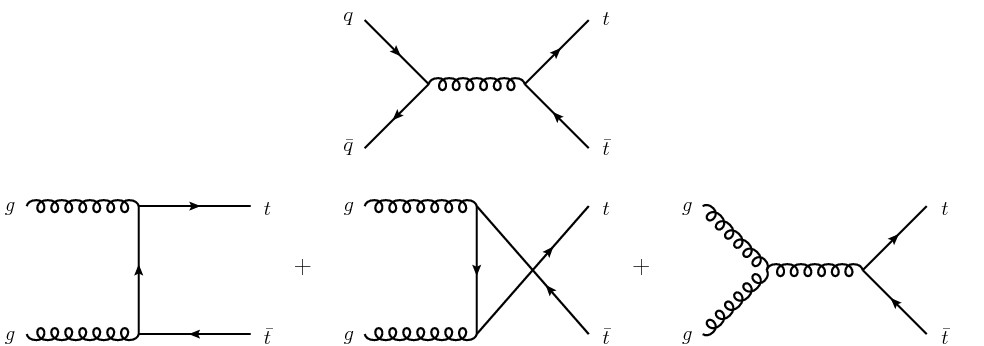
\includegraphics[width=0.97\textwidth]{figs/top-physics/ttbar_feyn.jpg}
\caption{The three Leading Order Feynman diagrams for top quark pair production at hadron colliders. Quark-anti quark annihilation is illustrated on the top row and gluon fusion on the bottom. Gluon fusion is the main production mode at the LHC and quark fusion at the Tevatron.}
\label{fig:feyn_ttbar}
\end{center}
\end{figure}

\editComment{Cross sections table} 

Top quark pair production can also occur in association with a vector boson, albeit at relatively small cross sections compared to both \ttbar and singly produced top quarks.
Despite their cross sections, these channels are important backgrounds which require detailed understanding in order to be able to probe for new physics with similar or smaller cross sections, such as \ttH or tZq~\cite{Khachatryan:2014ewa}.

\subsection{Single top quark production}\label{subsec:singleTopTheory}
Top quarks can also be produced singly through weak interactions, albeit with smaller cross sections than \ttbar given the relative weakness of the electroweak coupling compared to the strong coupling.

Such processes are an powerful probe between the top and electroweak sector of the SM.
The Wtb vertex allows for the direct measurement of the $\abs{V_{tb}}$ element of the Cabibbo-Kobayashi-Maskawa (CKM) matrix and thus test whether the CKM matrix is unitary as presumed or otherwise~\cite{Shibata:2008sy}.
Additionally, these processes can be used to determine the top quark's spin by considering the angular distribution of its decay products.

Understanding single top quark processes is also important from an experimental viewpoint as:
\begin{itemize}
\item these processes form backgrounds for not only SM processes such as \ttbar, but for for Higgs and BSM physics searches, such as anomalous couplings.
\item precision measurements of these processes can be used to constrain Parton Distribution Functions~\cite{Guffanti:2010yu}.
\end{itemize}

The main SM single top production mechanisms are categorised by the virtuality of the W boson involved in the interaction.
As each of these production channels have differing initial and final states they are typically considered separately.

\begin{figure}[!h]
\centering
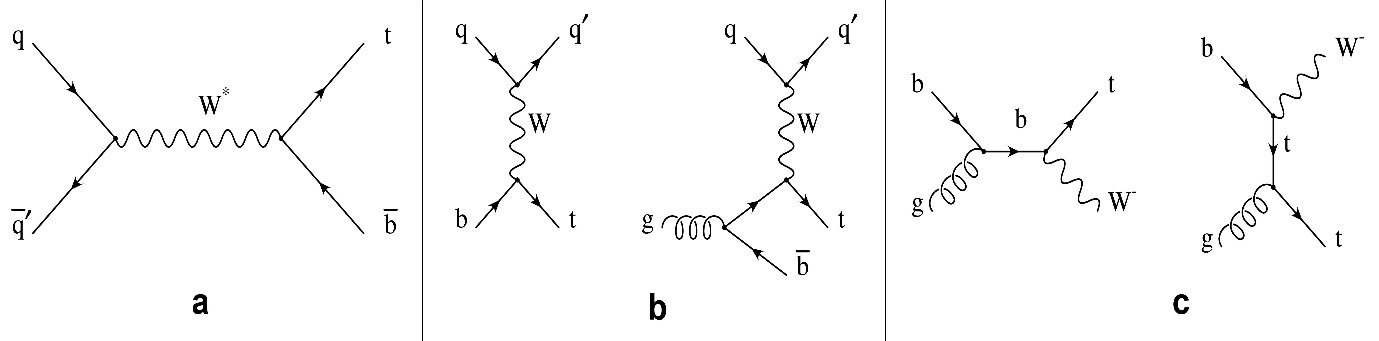
\includegraphics[width=1.00\textwidth]{figs/top-physics/singletop_feyn.jpg}
\caption{Leading order diagrams for single top quark production channels via weak processes: (a) s-channel, (b) t-channel and (c) tW.}
\label{fig:singleTopDiagrams}
\end{figure}

\editComment{Cross sections table} 

s-channel production, as shown in figure~\ref{fig:singleTopDiagrams}(a), is the quark anti-quark annihilation into an off-shell W boson which decays into a top and anti-bottom quark.
This process has the lowest single top production cross section at the LHC given the virtuality of the W boson required to produce the top quark and need for the anti-quark to originate from a sea quark.
Given its low cross section and a final state topology similar to larger background processes, the s-channel has yet to be observed at the LHC~\cite{Khachatryan:2016ewo}.

The t-channel, as shown in figure~\ref{fig:singleTopDiagrams}(b), is the dominant single top prodution mechanism at the LHC.
The process involves the scattering of the W boson off a bottom quark originating either from a sea quark or from gluon splitting.
Initially observed at the Tevatron~\cite{Aaltonen:2009jj,Abazov:2009ii}, the t-channel has since been studied at higher energies at the LHC, with all results to date remaining consistent with the SM~\cite{Berta:2017ghf,Morton:2018wkb}.	

The tW-channel, as shown in figure~\ref{fig:singleTopDiagrams}(c), is where a top quark is produced in association with an on-shell W boson.
In contrast to being negligible at the Tevatron, the tW-channel is accessible at LHC and was discovered in 2014~\cite{Chatrchyan:2014tua}.
The discovery of the tW-channel was particularly anticipated as the presence of the on-shell W boson in the final state makes it an excellent probe of the Wtb vertex and the theoretical challenges that were involved in describing its interference with \ttbar production at next-to-leading order.

\subsection{Single top production in association with a Z boson}\label{subsec:tZqTheory}
With the high centre-of-mass energies and integrated luminosities available at the LHC, it has become possible to not only undertake precision studies of singly and pair produced top quarks, but also to probe the top quark and electroweak sector.
Such measurements provide not only the ability to perform precision tests of SM predictions, but are also sensitive to new physics such as new electroweak bosons, new fermions, and Flavour Changing Neutral Currents (FCNC).

One may initially assume that given the larger production cross section for \ttbar compared to single top processes, that it would be considerably more difficult to probe the top-electroweak sector through single top quark production processes.
The top quark and W boson coupling however, can only be probed through the single top tW-channel given that the W boson couples to the initial state quarks for \ttW, as illustrated in figure~\ref{fig:feyn_ttV}.
tH has yet to be observed~\cite{CMS:2018jsz} as it is much more difficult to access than \ttH due to the destructive interference between the tH and HW vertices~\cite{Maltoni:2001hu}.
In contrast, \ttZ has a lower production cross section than the combined tZ and $\overline{\text{t}}$Z cross section~\cite{Campbell:2013yla}.
This is the result of the large number of particles present in the \ttZ final state suppressing \ttZ production despite the relative strength of the strong coupling.
CMS has made measurements of \ttH, \ttW, and \ttZ, all in excess of five standard deviations and consistent with their SM predictions~\cite{Sirunyan:2017uzs,Sirunyan:2018hoz}.

\begin{figure}[p]
\centering
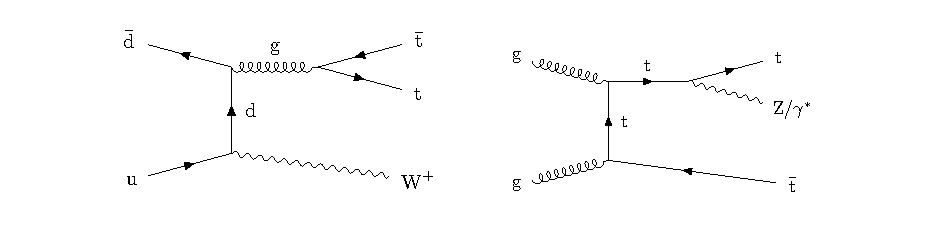
\includegraphics[width=\textwidth]{figs/top-physics/CMS-TOP-17-005_Figure_001.pdf}
\caption{Leading order \ttW (left) and \ttZ (right) production diagrams~\cite{Sirunyan:2017uzs}. Unlike for \ttZ and \ttH, the gauge boson in \ttW is not radiated from the top quark, but from the initial state quarks.}
\label{fig:deyn_ttV}
\end{figure}

The analysis presented in this thesis is the search for the production of a single top quark in association with a Z boson with an additional jet, known as \emph{tZq}, in the dilepton final state.
tZq is a rare SM process which provides a unique precision probe of the top quark and the electroweak sector, as the Z boson is radiated off one of the quark legs, as shown in figures~\ref{fig:feyn_tZq}(a)-(e), or from the exchanged W boson, as shown in figure~\ref{fig:feyn_tZq}(f).
Therefore, in contrast to \ttZ, tZq not only sensitive to the top quark and Z boson coupling, but also to the WWZ coupling.
In addition, tZq is an important process to be understood as it forms irreducible backgrounds for other rare SM processes, such as tH, but also BSM processes such as Flavour Changing Neutral Currents (FCNC)~\cite{AguilarSaavedra:2004wm}

\begin{figure}[p]
\centering
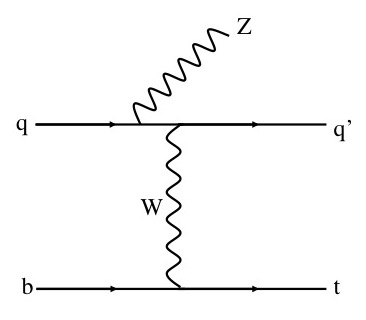
\includegraphics[width=0.47\textwidth]{figs/top-physics/tZq_feyn1.jpg}
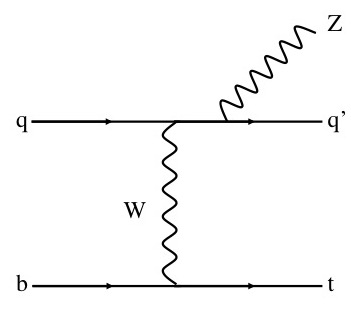
\includegraphics[width=0.47\textwidth]{figs/top-physics/tZq_feyn2.jpg}
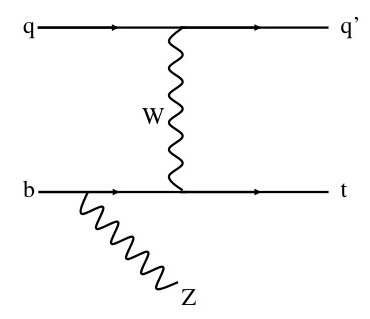
\includegraphics[width=0.47\textwidth]{figs/top-physics/tZq_feyn3.jpg}
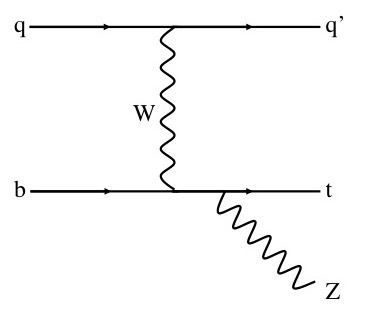
\includegraphics[width=0.47\textwidth]{figs/top-physics/tZq_feyn4.jpg}
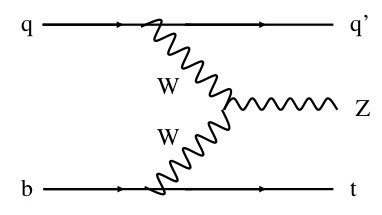
\includegraphics[width=0.47\textwidth]{figs/top-physics/tZq_feyn5.jpg}
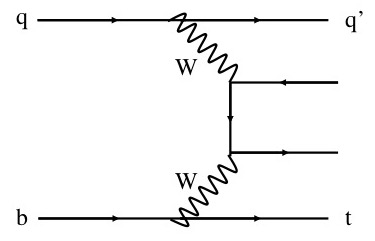
\includegraphics[width=0.47\textwidth]{figs/top-physics/tZq_feyn6.jpg}
\caption{Leading order tZq production diagrams, where the Z boson is radiated off one of the quark lines in (a)-(e) and from the the non-resonant contribution to the tqZ process from the W boson exchange in (f).}
\label{fig:feyn_tZq}
\end{figure}

The first search for tZq was undertaken for the fully leptonic final state using data collected by the CMS detector at $\sqrt{s} = 8\TeV$.
This final state involves the W boson from the top quark decay and the Z boson decaying leptonically and two or three jets, one from the bottom quark produced from the top quark decay, one from the recoil quark and potentially one from the gluon splitting that creates the initial state bottom quark.
While the trilepton final state has a smaller production cross section than either of the final states where the W boson or Z boson decays hadronically, it is the easiest to distinguish against background processes.

The first search for tZq however, was unable to observe the process, making a measurement with a significance of 2.9 standard deviations~\cite{Sirunyan:2017kkr}.
Both ATLAS and CMS have since been able to observe the trilepton final state for tZq at $\sqrt{s} = 13\TeV$ as a result of the Z and $\overline{\text{t}}$Z cross sections increasing with the centre-of-mass energy at a similar rate to \ttZ and the large integrated luminosity delivered by the LHC at $\sqrt{s} = 13\TeV$~\cite{Aaboud:2017ylb,Sirunyan:2017nbr}.

Such an increase in statistics has also made it possible to search for the other tZq final states, including the dilepton final state, where the Z boson decays leptonically and the W boson decays hadronically.
This final state involves the presence of two leptons consistent with a Z boson decay and at least four jets, with one being a bottom quark produced from the top quark decay, one from the recoil quark, and two from two quarks produced from the W boson decay.
Additional jets may be produced as the result of gluon splitting.
The full event selection requirements used in the analysis of this process is discussed in detail in Chapter~\ref{chapter:tzq-search}.

\begin{figure}[h]
\centering
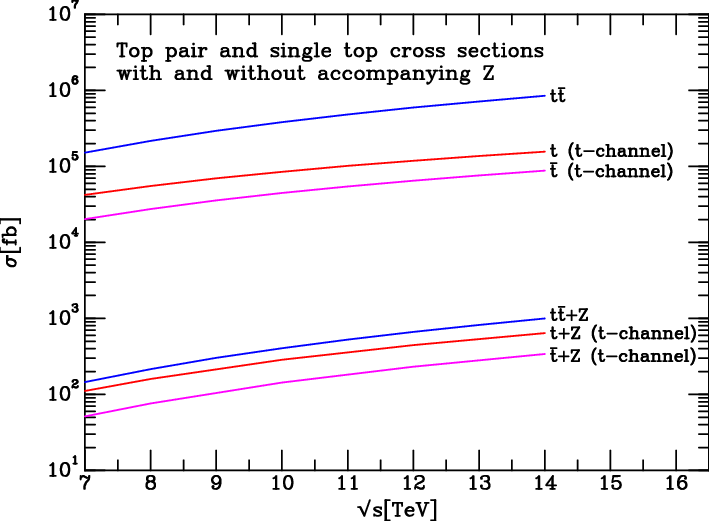
\includegraphics[width=\textwidth]{figs/top-physics/TplusZtot.png}
\caption{The next-to-leading order cross section for single top and top pair production with and without an associated Z boson as a function of the centre-of-energy for proton-proton collisions at the LHC~\cite{Campbell:2013yla}.
}
\label{fig:topZcrossSections}
\end{figure}

\section{Beyond the Standard Model Physics}\label{sec:bsm}
The SM has been incredibly successful at accurately predicting the majority of the properties of the known fundamental particles up to the electroweak scale.
Despite this however, given the inability of the SM to incorporate gravity and address a number of experimental observations, it is apparent that there must be physics Beyond the Standard Model (BSM).

\subsection{Shortcomings of the Standard Model Physics}\label{subsec:shortcomings}
One of the major and most apparent shortcomings of the SM is its inability to explain why there is an asymmetry between matter and anti-matter in the universe.
While CP violation does occur within the SM, it is insufficient to account for the degree of the matter excess observed.

Gravity currently is described by the extremely successful classical theory of General Relativity (GR).
GR however, is fundamentally incompatible with the SM and  has produced contradictory results such as the predicted cosmological constant and Higgs field's vacuum energy density.
While attempts have been made to reconcile the two theories, no successful quantum theory of gravity has been produced to date~\cite{Sola:2013gha}.	

One of the other serious theoretical issues with the SM is the so-called \emph{hierarchy problem} concerning the vast discrepancies between aspects of the weak force and gravity~\cite{Burdman:2007ck}.
As the vacuum expectation value of the Higgs field determines the mass of the weak bosons, for the observed masses of these bosons, one would expect a vacuum expectation value of approximately 246\GeV.
Given that the radiative corrections to the observable mass of the Higgs boson are proportional to the energy scale of new physics, this would imply that the Higgs vacuum expectation value would be either zero or of the order of the BSM physics energy scale.
In order to obtain the observed Higgs mass the cancellations required from the radiative corrections must be extremely ``fine tuned''.
While there is nothing fundamentally wrong with this, many scientists find such fine tuning to be \emph{unnatural}.

Other astronomical and cosmological inconsistencies include the presence of \emph{dark matter} (DM) and \emph{dark energy} in the universe.
The observations of the rotation of galaxies, gravitational lensing, structure of the universe and the Cosmic Microwave background, indicates that there must be a form of ``dark'' matter present~\cite{Aghanim:2018eyx}.
The accelerating expansion of the universe is also unaccounted for and implies the existence of a ``dark energy'' to drive this~\cite{Peebles:2002gy,Aghanim:2018eyx}.

Perhaps the greatest inconsistency experimentally observed with the SM is that of massive neutrinos.
The first indication of massive neutrinos was made by the ``Homestake'' experiment which found that the fraction of electron neutrinos arriving from the Sun was at the most half (if not less) what was expected~\cite{PhysRevLett.20.1205}.
While this observation could be explained by neutrinos experiencing flavour oscillations, this would require neutrinos to have mass in contrast to the SM in order for their flavour eigenstates to mix with their mass eigenstates.
Further experiments have confirmed however, that neutrinos do experience flavour oscillations as they propagate through space and thus must have mass~\cite{Fukuda:1998mi,Ahmad:2001an,PhysRevD.88.032002}.

\subsection{Flavour Changing Neutral Currents}\label{sec:fcncs}
Given the limited experimental evidence of BSM physics, a large number of BSM physics models, driven by theoretical and ascetic arguments, have been proposed to account for the shortcomings of the SM.
While the analysis presented in this thesis concerns the search for a SM process, the tZq cross section is sensitive to modifications of the tZ coupling posited by a number of BSM theories.

As discussed in Chapter~\ref{}, in the SM any FCNC process that changes a quark's flavour but not its charge must be loop mediated.
A number of BSM theories however, introduce top quark FCNC decay contributions at the tree level, such as Supersymmetry (SUSY) models and those proposing additional Higgs doublets and/or quark singlets~\cite{AguilarSaavedra:2004wm}.
The presence of such new tZ couplings would enhance the production rate of both \ttZ and tZq by several orders of magnitude and should be observable at the LHC. 
As of to date however, no evidence for BSM FCNCs have been observed for the tZ coupling for both single top and \ttbar processes~\cite{Sirunyan:2with017kkr}.
